%
% Portuguese-BR vertion
% 
\documentclass{report}

\usepackage{ipprocess}
% Use longtable if you want big tables to split over multiple pages.
\usepackage{longtable}
\usepackage[utf8]{inputenc}
\usepackage[brazil]{babel} % Uncomment for portuguese

\sloppy

\graphicspath{{./pictures/}} % Pictures dir
\makeindex

\begin{document}

\DocumentTitle{Documento de Arquitetura}
\Project{Core-MUSA}
\Organization{Universidade Estadual de Feira de Santana}
\Version{Build 2.0a}

\capa
\newpage
\newpage

%%%%%%%%%%%%%%%%%%%%%%%%%%%%%%%%%%%%%%%%%%%%%%%%%%
%% Revision History
%%%%%%%%%%%%%%%%%%%%%%%%%%%%%%%%%%%%%%%%%%%%%%%%%%
\chapter*{Histórico de Revisões}
  \vspace*{1cm}
  \begin{table}[ht]
    \centering
    \begin{tabular}[pos]{|m{2cm} | m{8cm} | m{4cm}|} 
      \hline
      \cellcolor[gray]{0.9}
      \textbf{Date} & \cellcolor[gray]{0.9}\textbf{Descrição} & \cellcolor[gray]{0.9}\textbf{Autor(s)}\\
      \hline 20/10/2014 &  Concepção do Documento & fmbboaventura \\ \hline
      		 23/10/2014 &  Revisão Inicial & jadsonfirmo \\ \hline
      		 29/10/2014 &  Adicionada Breve Descrição dos Componentes & fmbboaventura \\ \hline       
      		 29/10/2014 & Stakeholders & jadsonfirmo \\ \hline
      		 30/10/2014 & Ajustes estruturais & fmbboaventura e jadsonfirmo \\ \hline
      		 30/10/2014 & Detalhamento das Instruções & jadsonfirmo, KelCarmo e Odivio \\ \hline
      		 30/10/2014 & Adição dos diagramas de classes & gordinh \\ \hline
      		 06/11/2014 & Mudanças nos Layouts das Instruções e no diagrama de classe da ULA & jadsonfirmo e KelCarmo \\ \hline
      		 10/11/2014 & Detalhamento dos Opcodes & jadsonfirmo \\ \hline
      		 13/11/2014 & Alteração na tabela dos Opcodes & jadsonfirmo \\ \hline
      		 17/11/2014 & Alteração no diagrama de classes da ULA e ajustes na tabela dos Opcodes & jadsonfirmo \\ \hline
      		 18/11/2014 & Ajustes dos Opcodes & jadsonfirmo \\ \hline
 		     24/11/2014 & Refatoração do DataPath & Odivio Caio \\ \hline
		  	 07/12/2014 & Opcodes de acordo com o Vênus & jadsonfirmo \\ \hline
		  	 07/12/2014 & Alteraçao Layout do JR e ajustes de conflitos & jadsonfirmo \\ \hline
		  	 08/12/2014 & Revisão documento de arquitetura & jadsonfirmo \\ \hline
    \end{tabular}
  \end{table}

% TOC instantiation
\tableofcontents

%%%%%%%%%%%%%%%%%%%%%%%%%%%%%%%%%%%%%%%%%%%%%%%%%%
%% Document main content
%%%%%%%%%%%%%%%%%%%%%%%%%%%%%%%%%%%%%%%%%%%%%%%%%%
\chapter{Introdução}
  
  \section{Propósito do Documento}
  Este documento descreve a arquitetura do projeto \ipPROCESSProject, incluindo especificações dos circuitos internos e máquinas de estados de cada componente. Ele também apresenta diagramas de classe, definições de entrada e saída e diagramas de temporização. O principal objetivo deste documento é definir as especificações do projeto \ipPROCESSProject\ e prover uma visão geral completa do mesmo.
  
%%%%%%%%%%%%%%%%%%%%%%%%%%%%%%
%  \noindent \textcolor{red}{\textit{Informações adicionais podem ser incluídas nesta seção. Entretanto, via de regra, ela não deve se extender por muitos parágrafos.}}
%%%%%%%%%%%%%%%%%%%%%%%%%%%%%%
  \section{Stakeholders}
    \FloatBarrier
    \begin{table}[H] 
      \begin{center}
        \begin{tabular}[pos]{|m{6cm} | m{8cm}|} 
          \hline 
          \cellcolor[gray]{0.9}\textbf{Nome} & \cellcolor[gray]{0.9}\textbf{Papel/Responsabilidades} \\ \hline
          Diego Leite e Lucas Morais & Gerencia  \\ \hline
           Victor Figueiredo, Matheus Castro, Odivio Caio Santos e Kelvin Carmo & Desenvolvimento  \\ \hline
           Filipe Boaventura e Wagner Bittencourt & Implementação  \\ \hline
           Jadson Firmo & Análise e Refatoração  \\ \hline
        \end{tabular}
      \end{center}
    \end{table} 

\section{Visão Geral do Documento}

O presente documento é apresentado como segue:\\

  \begin{itemize}
   \item \textbf{Capítulo 2 --} Este capítulo apresenta uma visão geral da arquitetura, com foco em entrada e saída do sistema e arquitetura geral do mesmo.
   \item \textbf{Capítulo 3 --} Este capítulo apresenta a descrição detalhada da arquitetura bem como seus módulos e componentes.
  \end{itemize}


  % inicio das definições do documento
  \section{Definições}
    \FloatBarrier
    \begin{table}[H]
      \begin{center}
        \begin{tabular}[pos]{|m{5cm} | m{9cm}|} 
          \hline
          \cellcolor[gray]{0.9}\textbf{Termo} & \cellcolor[gray]{0.9}\textbf{Descrição} \\ \hline
                          &                       \\ \hline
        \end{tabular}
      \end{center}
    \end{table}  
  % fim

  % inicio da tabela de acronimos e abreviacoes do documento
  \section{Acrônimos e Abreviações}
    \FloatBarrier
    \begin{table}[H]
      \begin{center}
        \begin{tabular}[pos]{|m{2cm} | m{12cm}|} 
          \hline
          \cellcolor[gray]{0.9}\textbf{Sigla} & \cellcolor[gray]{0.9}\textbf{Descrição} \\ \hline
             PC       &  Contador de Programa (Program Counter)\\ \hline
             ULA      &  Unidade Lógica e Aritmética\\ \hline
             OPCODE   &  Código da Operação\\ \hline
        \end{tabular}
      \end{center}
    \end{table}  
  % fim

\chapter{Visão Geral da Arquitetura}
  \section{Arquitetura geral MUSA}
  \begin{figure}[H]
	\centering
	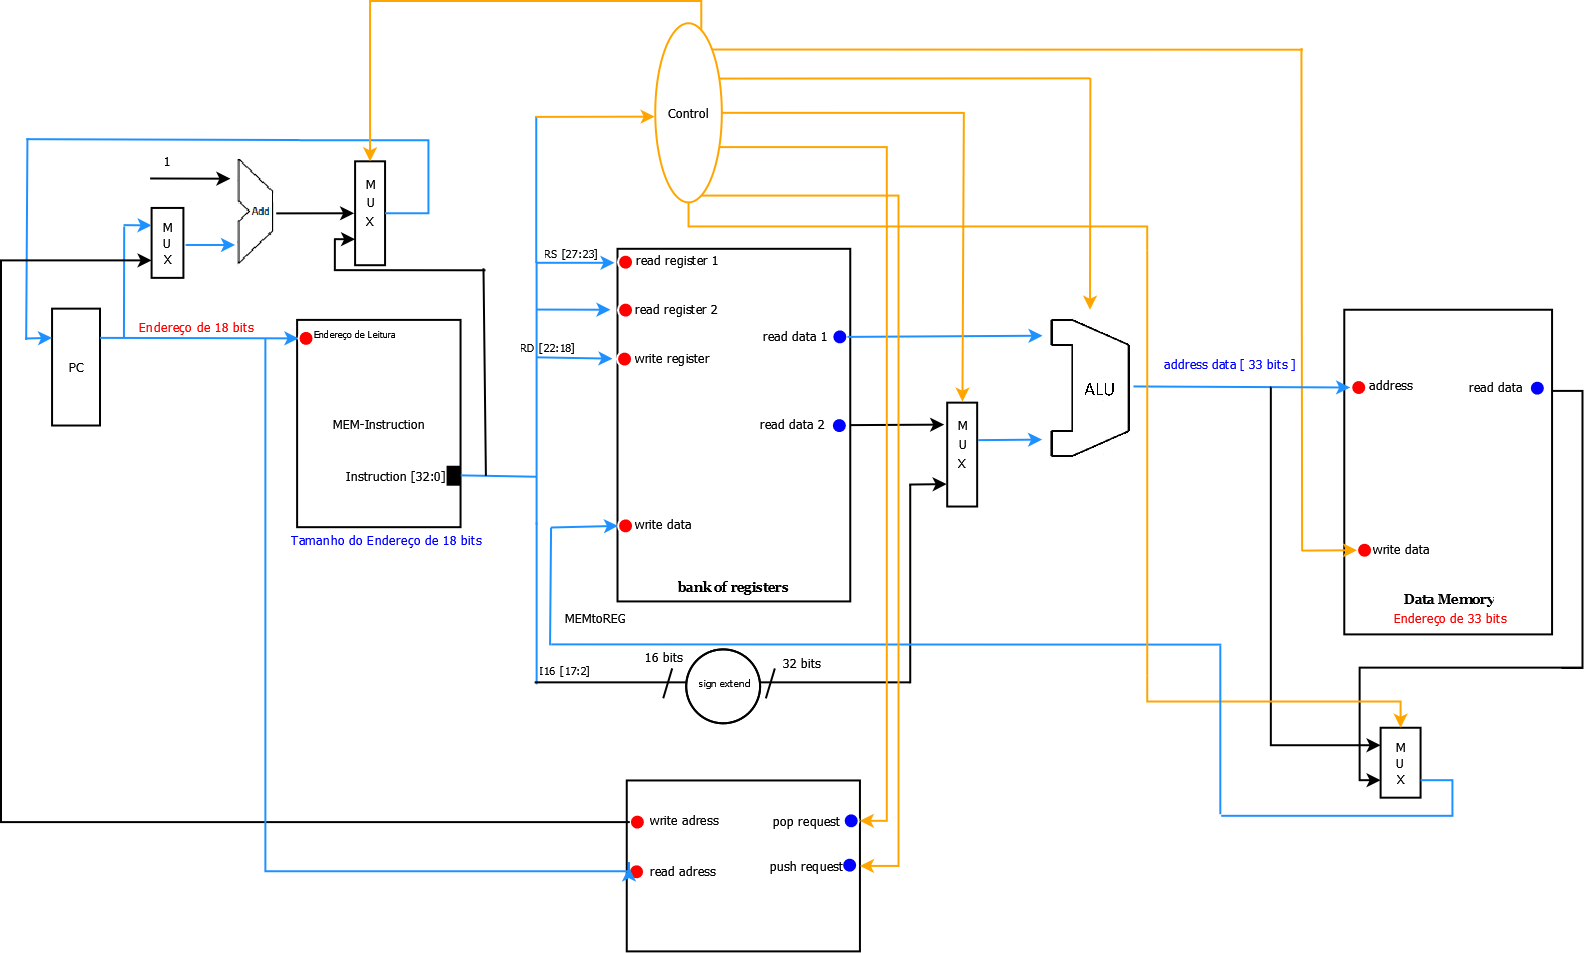
\includegraphics[width=\linewidth]{./pictures/DataPaths/Arquitetura/DataPathFinal.png}
  \end{figure}  

  \section{Descrição dos Componentes}
  A unidade de processamento a ser desenvolvida é composta a partir dos seguintes componentes:
  
  \begin{itemize}
    \item \textbf{PC --} Registrador que guarda o endereço da próxima instrução a ser executada.
    
    \item \textbf{Memória de Dados --} A Memória de dados é endereçada com 33 bits, que comporta no máximo 2 elevado a 33 palavras de instrução no total, que guarda dados com tamanho de 32 bits que foram manipulados pelo programa ou processador. 
   
    \item \textbf{Memória de Instrução --} A Memória de instrução é endereçada com 18 bits, que comporta no máximo 2 elevado a 18 palavras de instrução no total, tem tamanho de 1048576 bytes, justamente pelo fato da palavra de instrução ter 32 bits. Por fim é a memória que guarda o programa codificado em linguagem assembly.
    
    \item \textbf{ULA --} É responsável por todo o processamento realizado no processador, pois esta unidade executa as instruções lógicas e aritméticas.
    
    \item \textbf{Unidade de Controle --} Esta unidade decodifica a instrução e define sinais de controle como, sinais de leitura, escrita de memória e de registradores de armazenamento temporário interno e sinais de liberação de barramentos para endereço e dados e unidades funcionais. As unidades funcionais internas do processador são controladas por esta unidade de temporização e controle. Os determinados sinais de controle são enviados para as demais unidades após a decodificação de uma determinada instrução que partem do registrador de instrução ( IR ).
    
    \item \textbf{Banco de Registradores --} Contém os 32 registradores de propósito geral do processador.
    
    \item \textbf{Pilha --} Memória destinada para armazenamento dos endereços de retorno de chamadas de funções. Possui 32 registradores de 18 bits e um contador responsável por apontar o topo da pilha.
  \end{itemize}
  
  \section{Intruções}
  A unidade de processamento possui 21 instruções essenciais para o processamento das operações. Elas são desmembradas em quatro formatos: R-type, I-type, Load/Store e Jump.
  
  \begin{itemize}
    \item \textbf{R-type --} Operações lógicas e aritméticas.
    
	\begin{table}[H]
	\centering
	\begin{tabular}{|c|m{6cm}|c|c|}
  	\hline 
  	\textbf{INSTRUÇÃO} & \textbf{DESCRIÇÃO} & \textbf{OPCODE} & \textbf{FUNCTION} \\ 
  	\hline   	
  	ADD & Soma de dois valores. & 000000 & 100000 \\ \hline
  	SUB & Subtração de dois valores. & 000000 & 100010 \\ \hline
  	MUL & Multiplicação de dois valores. & 000000 & 011000 \\ \hline
  	DIV & Divisão de dois valores. & 000000 & 011010 \\ \hline
  	AND & Operação lógica AND entre dois valores. & 000000 & 100100 \\ \hline
  	OR & Operação lógica OR entre dois valores. & 000000 & 100101 \\ \hline
  	NOT & Operação lógica NOT. & 000000 & 100111 \\ \hline
  	CMP & Comparação de dois valores. & 000000 & 011011 \\ \hline
  	JR & Desvia o programa para um endereço de destino. & 001000 & - \\ \hline
  	\end{tabular} 
  	\caption{Instruções do tipo R.}
  \end{table}    

    \item \textbf{I-type --} Operações imediatas.
    
	\begin{table}[H]
	\centering
	\begin{tabular}{|c|m{6cm}|c|c|}
  	\hline 
  	\textbf{INSTRUÇÃO} & \textbf{DESCRIÇÃO} & \textbf{OPCODE} & \textbf{FUNCTION} \\ 
  	\hline 
  	ADDi &  Soma de dois valores, sendo um destes imediato. & 001000 & - \\ \hline
  	SUBi & Subtração de dois valores, sendo um destes imediato. & 001001 & - \\ \hline
  	ANDi & Operação lógica AND entre dois valores, sendo um destes imediato. & 001100 & - \\ \hline
  	ORi & Operação lógica OR entre dois valores, sendo um destes imediato. & 001101 & - \\ \hline
  	\end{tabular} 
  	\caption{Instruções do tipo I.}
  \end{table}

    \item \textbf{Load/Store --} Operações de carregamento e armazenamento (Intruções de tipo I).

	\begin{table}[H]
	\centering
	\begin{tabular}{|c|m{6cm}|c|c|}
  	\hline 
  	\textbf{INSTRUÇÃO} & \textbf{DESCRIÇÃO} & \textbf{OPCODE} & \textbf{FUNCTION} \\ 
  	\hline 
  	LW & Operação de leitura na memória de dados. & 100011 & - \\ \hline
  	SW & Operação de armazenamento na memória de dados. & 101011 & - \\ \hline
  	\end{tabular} 
  	\caption{Instruções de Load/Store.}
  \end{table}
    
    \item \textbf{Jump --} Operações de desvio e branch.
    
	\begin{table}[H]
	\centering
	\begin{tabular}{|c|m{6cm}|c|c|}
  	\hline 
  	\textbf{INSTRUÇÃO} & \textbf{DESCRIÇÃO} & \textbf{OPCODE} & \textbf{FUNCTION} \\ 
  	\hline 

  	JPC & Desvia o programa para um endereço relativo ao PC. & 001001 & - \\ \hline
  	BRFL & Desvia o programa para um endereço de destino, atendendo uma condição de flag. & 010001 & - \\ \hline
  	CALL & Desvia um programa em execução para uma sub-rotina. & 000011 & - \\ \hline
  	RET & Retorna de uma sub-rotina. & 000111 & - \\ \hline
  	HALT & Para a execução de um programa. & 000010 & - \\ \hline
  	NOP & Não realiza operação. & 000001 & - \\ \hline

  	\end{tabular} 
  	\caption{Instruções de Load/Store.}
  \end{table}
    
    \end{itemize}

  \section{Detalhamento das Intruções}
  
  \begin{itemize}
     
     \item \textbf{ADD, SUB, MUL, DIV, AND, OR, NOT e JR :}

  \begin{table}[H]
\centering
	\begin{tabular}{|c|c|c|c|c|c|}
  	\hline 
  	\textbf{OPCODE} & \textbf{RS} & \textbf{RT} & \textbf{RD} & \textbf{SHAMT} & \textbf{FUNCTION} \\ 
  	\hline 
  	06 & 05 & 05 & 05 & 05 & 06 \\ 
  	\hline 
  	\end{tabular} 
  	\caption{Instruções do tipo R.}
  \end{table}
  
  Esse conjunto de instruções utiliza dois registradores fontes (RS e RT) de dados e um registrador de destino (RD) para realizar as operações. O campo FUNCTION é utilizado como um segundo campo de código de operação, ampliando o leque de operações possíveis. O campo IM é reservado para as operações imediatas.\\
  
   \item \textbf{LW e SW, ADDi, SUBi, ANDi, ORi e BRFL:}

  \begin{table}[H]
\centering
	\begin{tabular}{|c|c|c|c|}
  	\hline 
  	\textbf{OPCODE} & \textbf{RD} & \textbf{RS} & \textbf{IMMEDIATE}  \\ 
  	\hline 
  	06 & 05 & 05 & 16 \\ 
  	\hline 
  	\end{tabular} 
  	\caption{Layout das Operações de Leitura/Escrita e operações imediatas}
  \end{table}
  
  Esse conjunto de instruções utiliza, além do código de operação (OPCODE), um registrador fonte (RS), e um registrador destino (RD) para instruções de leitura (LW) e de escrita (SW). Utiliza também do campo I (de 16 bits) que representa o deslocamento do registrador base. Os dois bits restantes serão sempre ignorados.\\

  
  \item \textbf{CALL, RET, HALT e NOP e JPC:}

  \begin{table}[H]
\centering
	\begin{tabular}{|c|c|}
  	\hline 
  	\textbf{OPCODE} & \textbf{TARGET} \\ 
  	\hline 
  	06 & 26 \\ 
  	\hline 
  	\end{tabular} 
  	\caption{Layout das Operações de Salto}
  \end{table}
  
  Instruções de salto, que especificam um registrador RF e uma CST (FLAG), para a instrução BRFL, que realiza um salto caso condição de comparação com a flag for verdadeira. Utilizará também 18 bits  utilizará 18 bits na instrução que respresenta uma posição de endereço de memória, para as instruções JR, CALL e HALT. As instruções RET e NOP só utilizam o OPCODE da instrução.\\
  
  \end{itemize}

% inicio das descrições de arquitetura para cada componente do sistema
\chapter{Descrição da Arquitetura}

  \section{ULA}

    \subsection{Diagrama de Classe}
    \begin{figure}[H]
	\centering
	\ucdiagram{./pictures/classes/ULA.png}
      \end{figure}      
     
    \subsection{Definições de Entrada e Saída}
      \FloatBarrier
      \begin{center}
        \begin{longtable}[pos]{| l | c | c | m{7cm} |} \hline         
          \multicolumn{1}{|c|}{\cellcolor[gray]{0.9}\textbf{Nome}} & 
          \multicolumn{1}{c|}{\cellcolor[gray]{0.9}\textbf{Tamanho}} & 
          \multicolumn{1}{c|}{\cellcolor[gray]{0.9}\textbf{Direção}} &
          \multicolumn{1}{c|}{\cellcolor[gray]{0.9}\textbf{Descrição}} \\ \hline
          \endfirsthead
          \hline
          \multicolumn{4}{|l|}%
          {{\bfseries continuação da página anterior}} \\
          \hline
          \multicolumn{1}{|c|}{\cellcolor[gray]{0.9}\textbf{Nome}} & 
          \multicolumn{1}{c|}{\cellcolor[gray]{0.9}\textbf{Tamanho}} & 
          \multicolumn{1}{c|}{\cellcolor[gray]{0.9}\textbf{Direção}} &
          \multicolumn{1}{c|}{\cellcolor[gray]{0.9}\textbf{Descrição}} \\ \hline
          \endhead

          \multicolumn{4}{|r|}{{continua na próxima página}} \\ \hline
          \endfoot

          \hline
          \endlastfoot

          clock                & 1   & entrada   & Sinal de clock da fase.    \\ \hline
          OP1             & 32   & entrada   & Valor do primeiro operando.    \\ \hline
          OP2             & 32   & entrada   & Valor do segundo operando.    \\ \hline
          Function             & 3   & entrada   & Identificador da operação.    \\ \hline
          Result             & 32   & saída   & Valor do resultado da operação realizada.    \\ \hline
          Overflow             & 1   & saída   & Sinal de overflow, para quando ocorrer overflow durante a operação.    \\ \hline
          Equals             & 1   & saída   & Sinal de igualdade, para quando ocorrer uma comparação entre dois valores iguais.    \\ \hline
        \end{longtable}
      \end{center}  
  %%%%%%%%%%%%%%%%%%%%%%%%%%%%%%%%%%%%%%%%%%%%%%
  \section{Busca de Instrução}

    \subsection{Diagrama de Classe}
    \begin{figure}[H]
	\centering
	\ucdiagram{./pictures/classes/Busca_de_Instrucao.png}
      \end{figure}      
     
    \subsection{Definições de Entrada e Saída}
      \FloatBarrier
      \begin{center}
        \begin{longtable}[pos]{| l | c | c | m{7cm} |} \hline         
          \multicolumn{1}{|c|}{\cellcolor[gray]{0.9}\textbf{Nome}} & 
          \multicolumn{1}{c|}{\cellcolor[gray]{0.9}\textbf{Tamanho}} & 
          \multicolumn{1}{c|}{\cellcolor[gray]{0.9}\textbf{Direção}} &
          \multicolumn{1}{c|}{\cellcolor[gray]{0.9}\textbf{Descrição}} \\ \hline
          \endfirsthead
          \hline
          \multicolumn{4}{|l|}%
          {{\bfseries continuação da página anterior}} \\
          \hline
          \multicolumn{1}{|c|}{\cellcolor[gray]{0.9}\textbf{Nome}} & 
          \multicolumn{1}{c|}{\cellcolor[gray]{0.9}\textbf{Tamanho}} & 
          \multicolumn{1}{c|}{\cellcolor[gray]{0.9}\textbf{Direção}} &
          \multicolumn{1}{c|}{\cellcolor[gray]{0.9}\textbf{Descrição}} \\ \hline
          \endhead

          \multicolumn{4}{|r|}{{continua na próxima página}} \\ \hline
          \endfoot

          \hline
          \endlastfoot

          clock\_in                & 1   & entrada   & Sinal de clock da fase.    \\ \hline
          entradaPC             & 18   & entrada   & Endereço do PC atual.    \\ \hline
          saidaInstrucao             & 32   & saída   & Instrução que sai da memória de instrução .    \\ \hline
        \end{longtable}
      \end{center}  
%%%%%%%%%%%%%%%%%%%%%%%%%%%%%%%%%%%%%%%%%%%%%%
  \section{Pilha}

    \subsection{Diagrama de Classe}
      \begin{figure}[H]
	\centering
	\ucdiagram{./pictures/classes/pilha.png}
      \end{figure} 
     
    \subsection{Definições de Entrada e Saída}
      \FloatBarrier
      \begin{center}
        \begin{longtable}[pos]{| l | c | c | m{7cm} |} \hline         
          \multicolumn{1}{|c|}{\cellcolor[gray]{0.9}\textbf{Nome}} & 
          \multicolumn{1}{c|}{\cellcolor[gray]{0.9}\textbf{Tamanho}} & 
          \multicolumn{1}{c|}{\cellcolor[gray]{0.9}\textbf{Direção}} &
          \multicolumn{1}{c|}{\cellcolor[gray]{0.9}\textbf{Descrição}} \\ \hline
          \endfirsthead
          \hline
          \multicolumn{4}{|l|}%
          {{\bfseries continuação da página anterior}} \\
          \hline
          \multicolumn{1}{|c|}{\cellcolor[gray]{0.9}\textbf{Nome}} & 
          \multicolumn{1}{c|}{\cellcolor[gray]{0.9}\textbf{Tamanho}} & 
          \multicolumn{1}{c|}{\cellcolor[gray]{0.9}\textbf{Direção}} &
          \multicolumn{1}{c|}{\cellcolor[gray]{0.9}\textbf{Descrição}} \\ \hline
          \endhead

          \multicolumn{4}{|r|}{{continua na próxima página}} \\ \hline
          \endfoot

          \hline
          \endlastfoot

          clock\_in                & 1   & entrada   & Sinal de clock da fase.    \\ \hline
          entradaDeDados             & 18   & entrada   & Endereço do PC que será armazenado.    \\ \hline
          popRequest             & 1   & entrada   & Sinal para tirar o ultimo endereço armmazenado da pilha.    \\ \hline
          pushRequest             & 1   & entrada   & Sinal para salvar o endereço do PC da pilha.    \\ \hline
          saidaDeDados             & 32   & saída   & Ultimo endereço salvo na pilha para retorno do PC.    \\ \hline
        \end{longtable}
      \end{center}  

%%%%%%%%%%%%%%%%%%%%%%%%%%%%%%%%%%%%%%%%%%%%%%
  \section{Acesso à memória}

    \subsection{Diagrama de Classe}
      \begin{figure}[H]
	\centering
	\ucdiagram{./pictures/classes/Leitura.png}
      \end{figure} 
     
    \subsection{Definições de Entrada e Saída}
      \FloatBarrier
      \begin{center}
        \begin{longtable}[pos]{| l | c | c | m{7cm} |} \hline         
          \multicolumn{1}{|c|}{\cellcolor[gray]{0.9}\textbf{Nome}} & 
          \multicolumn{1}{c|}{\cellcolor[gray]{0.9}\textbf{Tamanho}} & 
          \multicolumn{1}{c|}{\cellcolor[gray]{0.9}\textbf{Direção}} &
          \multicolumn{1}{c|}{\cellcolor[gray]{0.9}\textbf{Descrição}} \\ \hline
          \endfirsthead
          \hline
          \multicolumn{4}{|l|}%
          {{\bfseries continuação da página anterior}} \\
          \hline
          \multicolumn{1}{|c|}{\cellcolor[gray]{0.9}\textbf{Nome}} & 
          \multicolumn{1}{c|}{\cellcolor[gray]{0.9}\textbf{Tamanho}} & 
          \multicolumn{1}{c|}{\cellcolor[gray]{0.9}\textbf{Direção}} &
          \multicolumn{1}{c|}{\cellcolor[gray]{0.9}\textbf{Descrição}} \\ \hline
          \endhead

          \multicolumn{4}{|r|}{{continua na próxima página}} \\ \hline
          \endfoot

          \hline
          \endlastfoot

          clock\_in                & 1   & entrada   & Sinal de clock da fase.    \\ \hline
          entradaDeDados             & 32   & entrada   & Valor que será armazenado na memória de dados.    \\ \hline
          AtivaEscrita             & 1   & entrada   & Sinal para ativar a escrita na memória de dados.    \\ \hline
          AtivaLeitura             & 1   & entrada   & Sinal para ativar a leitura na memória de dados.    \\ \hline
          saidaDeDados             & 32   & saída   & Valor que irá sair da memória de dados.    \\ \hline
        \end{longtable}
      \end{center}  
   
%%%%%%%%%%%%%%%%%%%%%%%%%%%%%%%%%%%%%%%%%%%%%%
  \section{Busca de Registradores}

    \subsection{Diagrama de Classe}
      \begin{figure}[H]
	\centering
	%\input{./pictures/classes/Registrador.png}
      \end{figure} 
     
    \subsection{Definições de Entrada e Saída}
      \FloatBarrier
      \begin{center}
        \begin{longtable}[pos]{| l | c | c | m{7cm} |} \hline         
          \multicolumn{1}{|c|}{\cellcolor[gray]{0.9}\textbf{Nome}} & 
          \multicolumn{1}{c|}{\cellcolor[gray]{0.9}\textbf{Tamanho}} & 
          \multicolumn{1}{c|}{\cellcolor[gray]{0.9}\textbf{Direção}} &
          \multicolumn{1}{c|}{\cellcolor[gray]{0.9}\textbf{Descrição}} \\ \hline
          \endfirsthead
          \hline
          \multicolumn{4}{|l|}%
          {{\bfseries continuação da página anterior}} \\
          \hline
          \multicolumn{1}{|c|}{\cellcolor[gray]{0.9}\textbf{Nome}} & 
          \multicolumn{1}{c|}{\cellcolor[gray]{0.9}\textbf{Tamanho}} & 
          \multicolumn{1}{c|}{\cellcolor[gray]{0.9}\textbf{Direção}} &
          \multicolumn{1}{c|}{\cellcolor[gray]{0.9}\textbf{Descrição}} \\ \hline
          \endhead

          \multicolumn{4}{|r|}{{continua na próxima página}} \\ \hline
          \endfoot

          \hline
          \endlastfoot

          clock\_in                & 1   & entrada   & Sinal de clock da fase.    \\ \hline
          EscritaDestino             & 32   & entrada   & Escrita do valor nos registradores de destino.    \\ \hline
          AtivaEscrita             & 1   & entrada   & Sinal para ativar a escrita no Banco de Registradores.    \\ \hline
          AtivaLeitura             & 1   & entrada   & Sinal para ativar a leitura no Banco de Registradores.    \\ \hline
          RegistradorDeSaida             & 32   & saída   & Saída do valor contido nos registradores.    \\ \hline
          RegistradorDestino             & 5   & Entrada   & Endereço do registrador destino.    \\ \hline
        \end{longtable}
      \end{center}  
% Optional bibliography section
% To use bibliograpy, first provide the ipprocess.bib file on the root folder.
% \bibliographystyle{ieeetr}
% \bibliography{ipprocess}

\end{document}
